\documentclass[msthesis.tex]{subfiles}

\begin{document}
\chapter{Results}
\section{Connectome Generation}

The 5TT image cannot be easily visualized in three dimensions. This problem was solved by estimating the response functions for multi-shell, multi-tissue constrained spherical deconvolution (MSMT-CSD)  based on the algorithm in \cite{jeurissen2014multi}. After obtaining three different files, each consisting of the response functions from the WM, GM and CSF separately, MSMT-CSD is performed to obtain fiber orientation distributions. It generates three different volumes which are then combined to generate a 4D image. In this 4D image, each volume represents the corresponding tissue densities of WM, GM and CSF. The 4D image is then visualized as an RGB image with each volume getting its specific color (Fig. \ref{fig:preproc}(b)).
\label{subsec:connectome_generation}
\begin{figure}
    \centering
    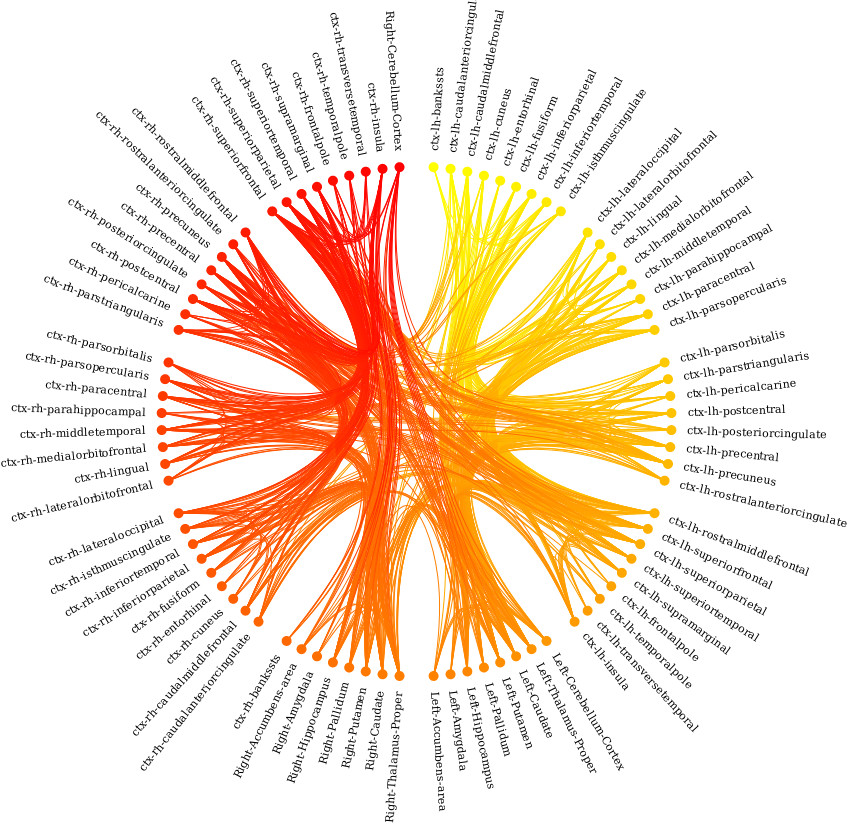
\includegraphics[width=\textwidth]{images/brain-data-viewer_2.png}
    \caption{Connectome of one subject with the mean streamline length visualized using tool connectome toolkit Neuromarvl \href{}{\textit{\textbf{https://immersive.erc.monash.edu/neuromarvl/}}}. The nodes of the connectome are represented on the end of the circle and are lablled according to the Desikan Killiany Atlas. The edges represent the connections between the different ROIs and are colored according the nodes they run between.}
    \label{fig:my_label}
\end{figure}

The connectome obtained was 84x84 upper triangular since the connections between the regions are to be considered as undirected. 
\begin{figure}
    \centering
    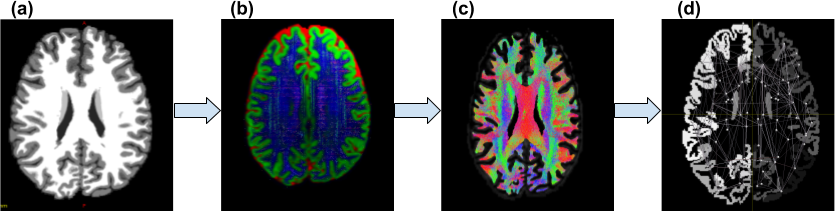
\includegraphics[width=\textwidth]{images/Preprocessing_pipeline.png}
    %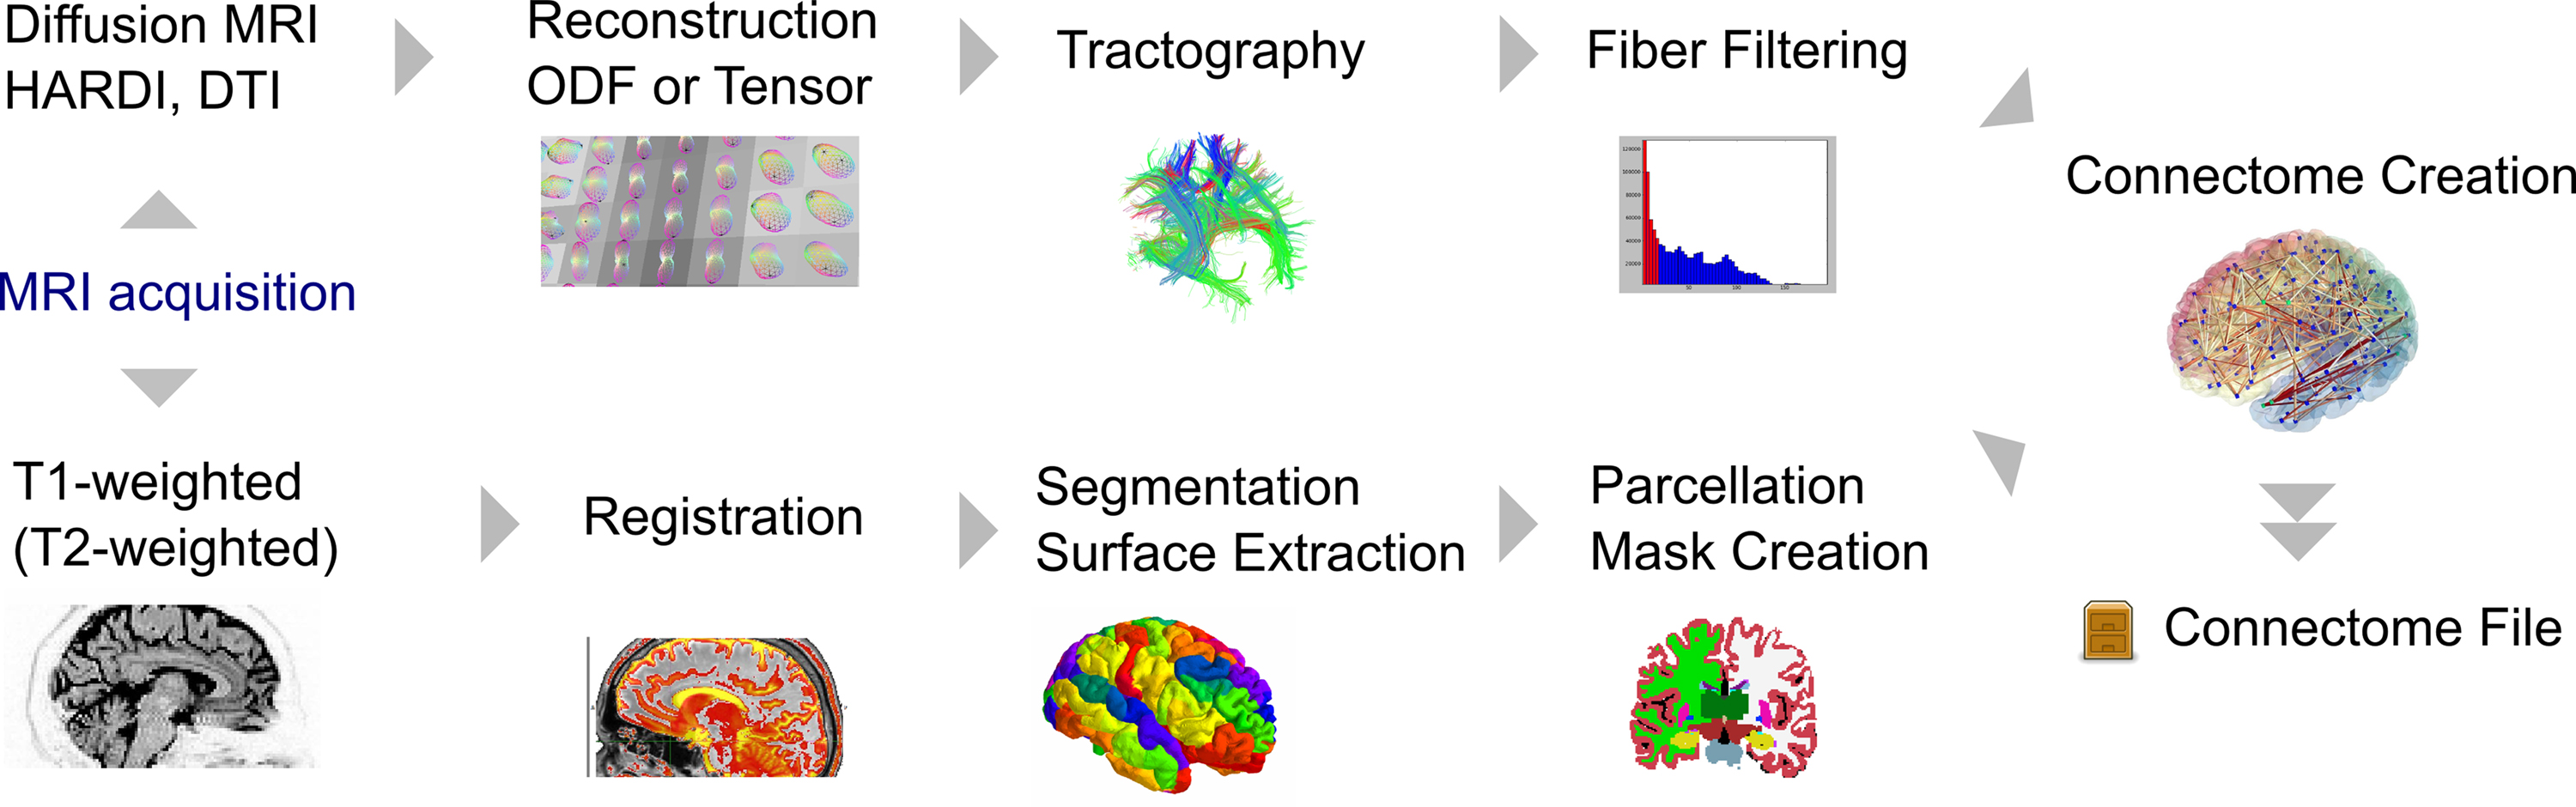
\includegraphics[width=\textwidth]{images/connectome_creation_workflow.png}
    %\cite{gerhard2011connectome}
    \caption{Visualization of pipeline used to create a connectome for each subject (a) Five tissue segmented image visualized in grayscale. (b) A slice of a 4D image mapped in 3D using RGB encoding tissue densities, CSF as red, GM as green and WM as blue. (c) Fiber tractography of 1M fibers produced using probabilistic tractography overlaid on an axial slice of the brain. (d) The nodes of the connectome representing ROIs overlaid on an axial slice}
    \label{fig:preproc}
\end{figure}
\section{Feature Representation Analysis}


\subsection{Self loops}
\label{res:selfloops}
\begin{table}
\csvreader[
  tabular=|c*{4}{|c}|,
  table head= \hline Train & Metric & Feature & T test & P value\\ \hline,
  late after last line=\\\hline,
]{tables/self_loops_test.csv}{}%
{\csvcoli & \csvcolii & \csvcoliii & \csvcoliv & \csvcolv }
\caption{Foo}
\end{table}
\subsection{Statistical Feature representation}



\section{Baseline analysis}
Comparing to no feature selection 100\% cases.
\begin{figure}
    \centering
    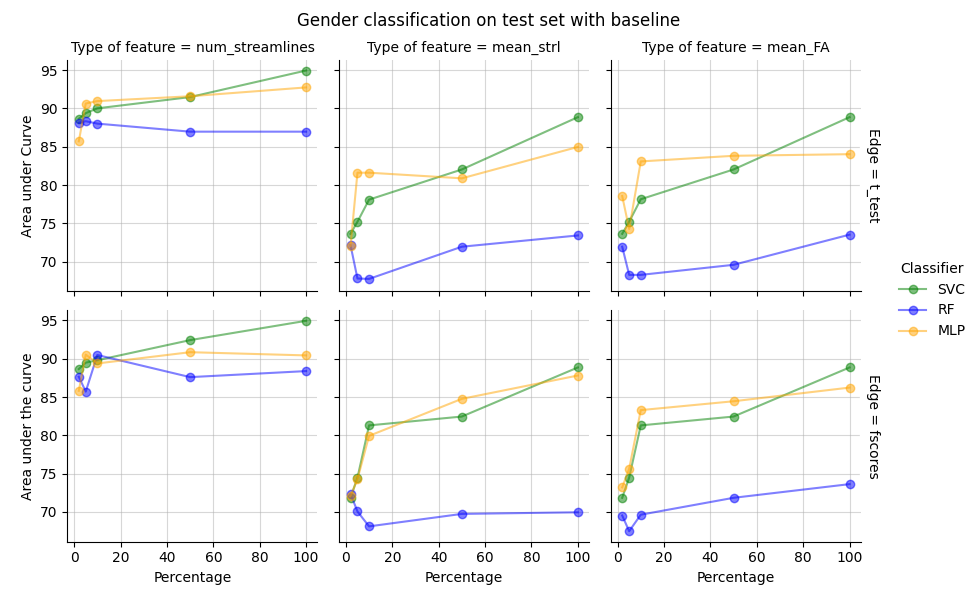
\includegraphics[width=\textwidth]{images/baseline_results_gender.png}
    \caption{Caption}
    \label{fig:my_label}
\end{figure}
\section{Solver Based Analysis}
\subsection{Input Graphs}
\subsubsection{Personality traits}

\subsection{Gender}
According to summary.csv,alyze how can we put it
After filtering according to the edges being selected only when there is atleast one streamline per subject. On the basis of the training subjects, the number of features for which all the subjects have a atleast one streamline with them is 1150. The input graph is hence formed on the basis of this with this number determining the upper bound of the number of edges in our inputgraph. 

\subsection{Output subgraphs}

- they are preserving x edges based on y nodes (specified, our condition was given to be true)
- connected
- subnet scores
- fscores and t-tests are giving similar results
\subsubsection{Personality traits}
\subsubsection{Gender}
\begin{figure}
    \centering
    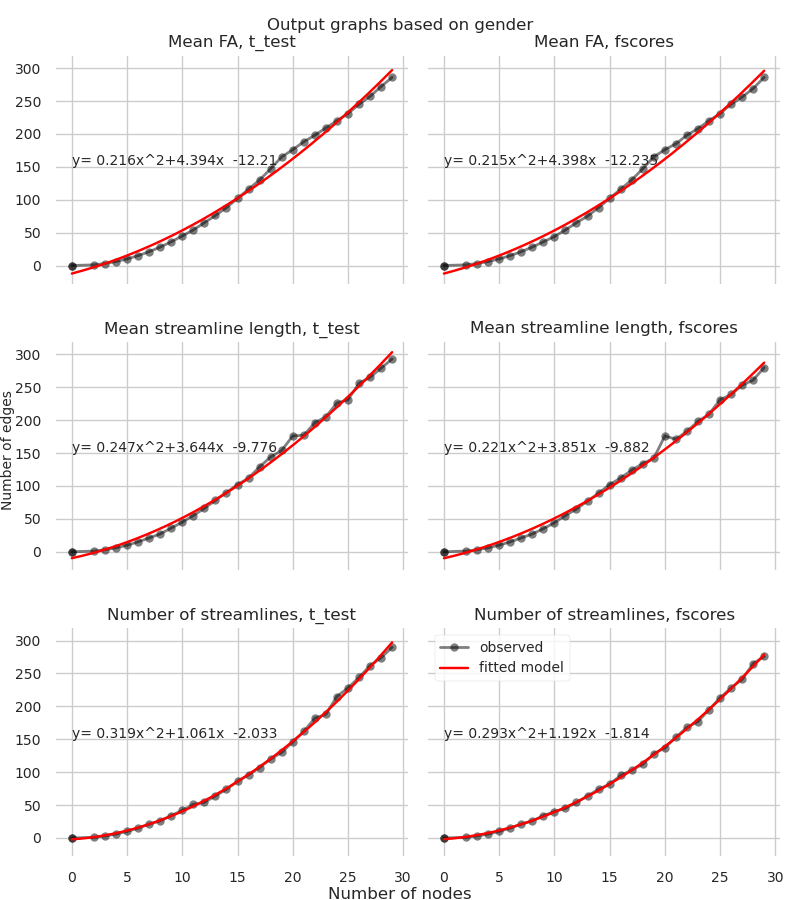
\includegraphics[width=0.8\textwidth]{images/Gender_nodes_preserved.png}
    \caption{Edges preserved as a function of nodes in the case of gender subgraph reduction}
    \label{fig:my_label}
\end{figure}



\section{Solver and baseline comparison}
\begin{figure}
    \centering
    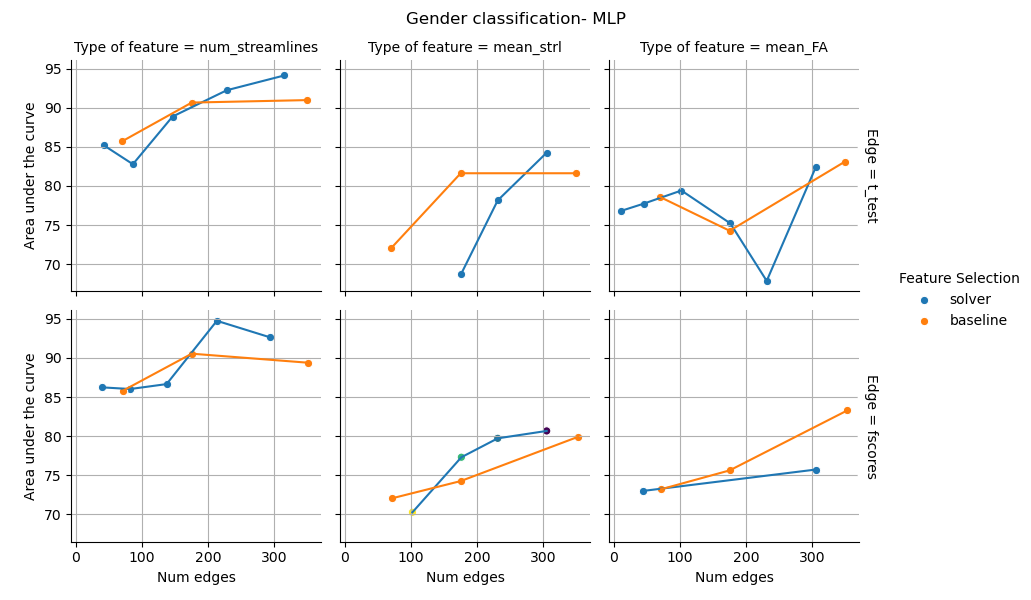
\includegraphics[width = \textwidth]{images/comparison_roc_auc_MLP.png}
    \caption{Caption}
    \label{fig:mlpgender}
\end{figure}
\begin{figure}
    \centering
    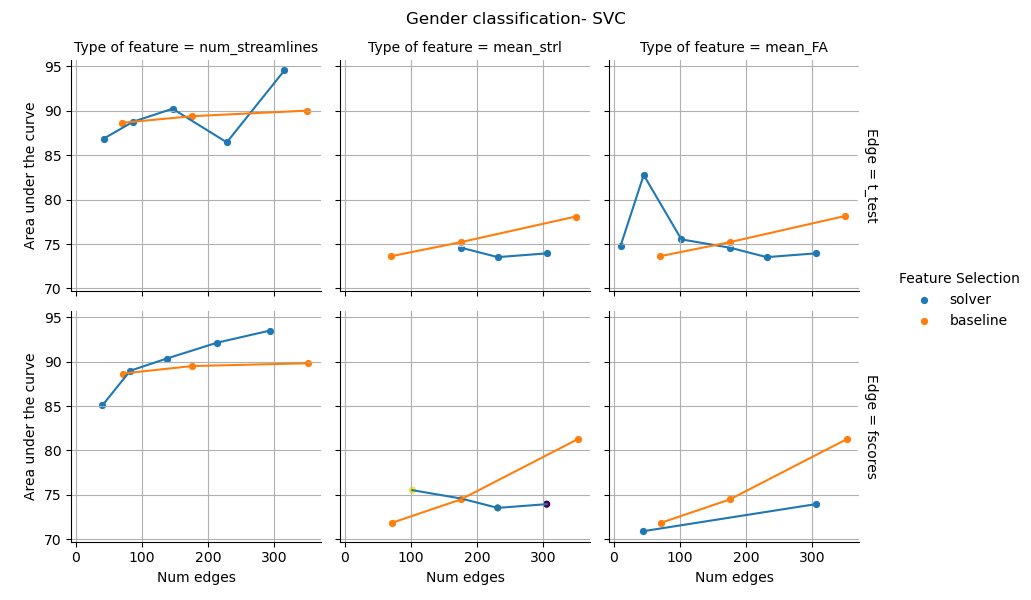
\includegraphics[width = \textwidth]{images/comparison_roc_auc_SVC.png}
    \caption{Caption}
    \label{fig:svcgender}
\end{figure}

\begin{figure}
    \centering
    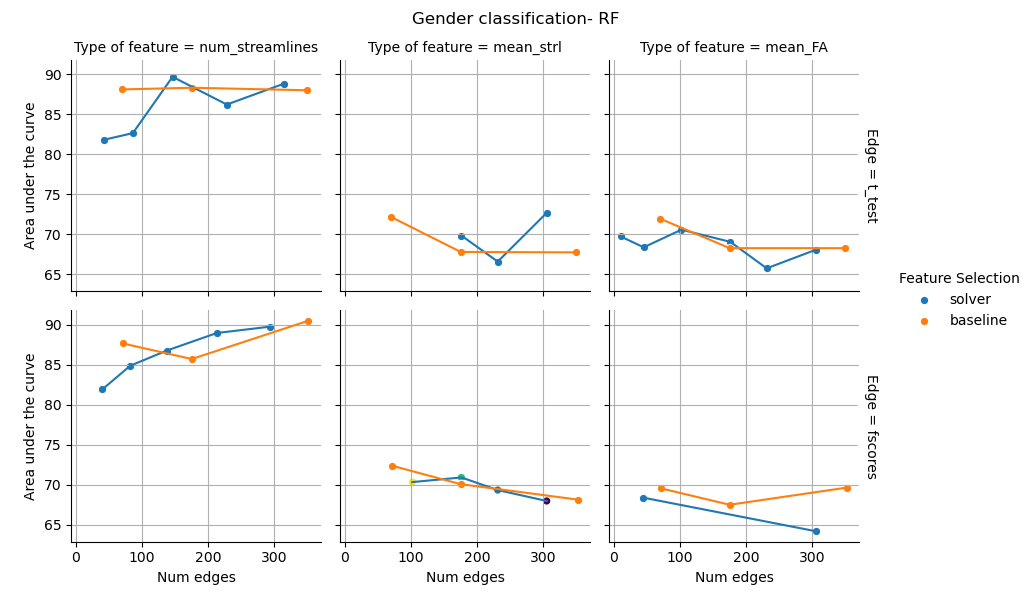
\includegraphics[width = \textwidth]{images/comparison_roc_auc_RF.png}
    \caption{Caption}
    \label{fig:rfgender}
\end{figure}

Judging on the basis of the area under the curve for gender based classification, it is best to compare feature wise.

Consider the mean FA feature first, for this feature the solver based approach does better than or equivalently well as the baseline when the number of edges preserved is small. This is not surprising since the number of edges preserved is a function of the number of nodes specified by the solver based technique. When a specified number of edges would be wanted to be preserved then the features corresponding to only those nodes will be preserved, this makes an inherent bias into which features will be preserved by the solver. Since all one node might have multiple highly relevant performance features but we want to preserve a given number of nodes, so the other less performing feature might be selected since a particular node has to be selected.


\begin{figure}
    \centering
    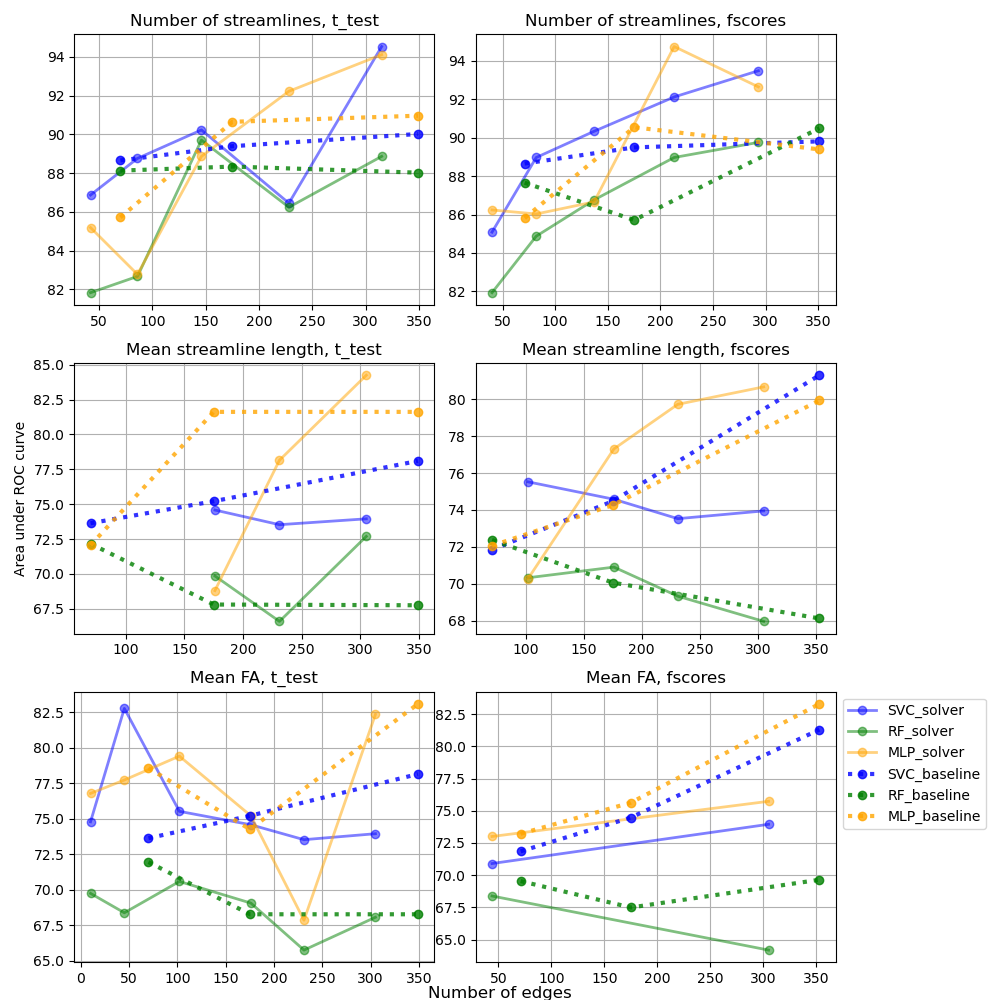
\includegraphics[width=\textwidth]{images/combined_clf_auc_gender.png}
    \caption{ Summary of Gender classification using baseline and solver techniques. In the figure with multiple subplots the rows represent the type of features used and the columns represent the type of edges used for feature ranking with the baseline analysis and as input graph representatives in the solver based approach. The y axis represents the area under the ROC curve for the classification on the test set as a function of the number of edges preserved by either techniques. Each time the number of nodes were specified in terms of percentages for the baseline implementation and as the number of nodes to be preserved for solver based implementation.}
    \label{fig:my_label}
\end{figure}

\section{Interpretabilitiy}

\end{document}
